\documentclass[12pt]{article}

% Core math
\usepackage{amsmath, amssymb, amsthm}
\usepackage{mathtools}

% Diagrams
\usepackage{tikz-cd}
\usepackage{tikz}
\usetikzlibrary{arrows, decorations.pathmorphing, positioning, calc, shapes.geometric, fit, backgrounds, chains}

% References and links
\usepackage{hyperref}
\usepackage{cleveref}

% Graphics
\usepackage{graphicx}

% Page layout
\usepackage[margin=1in]{geometry}

% Sidebar
\usepackage{everypage}
\usepackage{xcolor}
\usepackage{booktabs}
\usepackage{enumitem}

\hypersetup{
  colorlinks=true,
  linkcolor=blue!55!black,
  citecolor=blue!55!black,
  urlcolor=blue!55!black
}

% Theorem environments
\newtheorem{theorem}{Theorem}[section]
\newtheorem{proposition}[theorem]{Proposition}
\newtheorem{lemma}[theorem]{Lemma}
\newtheorem{corollary}[theorem]{Corollary}
\newtheorem{conjecture}[theorem]{Conjecture}
\theoremstyle{definition}
\newtheorem{definition}[theorem]{Definition}
\newtheorem{example}[theorem]{Example}
\theoremstyle{remark}
\newtheorem{remark}[theorem]{Remark}
\newtheorem{hook}[theorem]{Composition Hook}
\newtheorem{theme}[theorem]{Cross-cutting Theme}
\newtheorem{emerg}[theorem]{Emergent Property}

% cleveref naming: ensure references render correctly per environment
\crefname{theorem}{Theorem}{Theorems}
\Crefname{theorem}{Theorem}{Theorems}
\crefname{proposition}{Proposition}{Propositions}
\Crefname{proposition}{Proposition}{Propositions}
\crefname{lemma}{Lemma}{Lemmas}
\Crefname{lemma}{Lemma}{Lemmas}
\crefname{corollary}{Corollary}{Corollaries}
\Crefname{corollary}{Corollary}{Corollaries}
\crefname{conjecture}{Conjecture}{Conjectures}
\Crefname{conjecture}{Conjecture}{Conjectures}
\crefname{definition}{Definition}{Definitions}
\Crefname{definition}{Definition}{Definitions}
\crefname{example}{Example}{Examples}
\Crefname{example}{Example}{Examples}
\crefname{remark}{Remark}{Remarks}
\Crefname{remark}{Remark}{Remarks}
\crefname{hook}{Hook}{Hooks}
\Crefname{hook}{Hook}{Hooks}
\crefname{theme}{Theme}{Themes}
\Crefname{theme}{Theme}{Themes}
\crefname{emerg}{Emergent Property}{Emergent Properties}
\Crefname{emerg}{Emergent Property}{Emergent Properties}

% Macros
\newcommand{\C}{\mathcal{C}}
\newcommand{\D}{\mathcal{D}}
\newcommand{\E}{\mathcal{E}}
\newcommand{\Phys}{\mathbf{Phys}}
\newcommand{\Info}{\mathbf{Info}}
\newcommand{\Hilb}{\mathbf{Hilb}}
\newcommand{\FHilb}{\mathbf{FHilb}}
\newcommand{\Vect}{\mathbf{Vect}}
\newcommand{\Set}{\mathbf{Set}}
\newcommand{\Cob}{\mathbf{Cob}}
\newcommand{\Bord}{\mathbf{Bord}}
\newcommand{\Cat}{\mathbf{Cat}}
\newcommand{\Ham}{\mathbf{Ham}}
\newcommand{\Phase}{\mathbf{Phase}}
\newcommand{\Floq}{\mathbf{Floq}}
\newcommand{\InfoGeom}{\mathbf{InfoGeom}}
\newcommand{\Theory}{\mathbf{Theory}}
\newcommand{\Rep}{\mathbf{Rep}}
\newcommand{\QChan}{\mathbf{QChan}}
\newcommand{\op}{\mathrm{op}}
\newcommand{\id}{\mathrm{id}}
\newcommand{\Hom}{\mathrm{Hom}}
\newcommand{\End}{\mathrm{End}}
\newcommand{\Tr}{\mathrm{Tr}}
\newcommand{\Ob}{\mathrm{Ob}}
\newcommand{\AdS}{\mathrm{AdS}}
\newcommand{\CFT}{\mathrm{CFT}}
\newcommand{\Area}{\operatorname{Area}}
\newcommand{\BG}{\mathrm{B}G}
\newcommand{\Z}{\mathbb{Z}}
\newcommand{\R}{\mathbb{R}}
\newcommand{\enc}{\mathrm{enc}}
\newcommand{\Lift}{\mathrm{Lift}}
\newcommand{\HaPPY}{\textsc{HaPPY}}

% GrokRxiv sidebar
\definecolor{grokgray}{RGB}{110,110,110}
\AddEverypageHook{%
  \ifnum\value{page}=1
    \begin{tikzpicture}[remember picture, overlay]
      \node[
        rotate=90,
        anchor=south,
        font=\Large\sffamily\bfseries\color{grokgray},
        inner sep=0pt
      ] at ([xshift=38pt, yshift=0.52\paperheight]current page.south west)
      {GrokRxiv:2026.04.synthesis\quad
       [\,math-ph\,$\cap$\,hep-th\,]\quad
       30 Apr 2026};
    \end{tikzpicture}
  \fi
}

\title{Synthesis --- Modular Composition of\\
Information, Phase, Modulation, and Geometry}

\author{MagnetonIO Research \\
\textit{Emergent Spacetime Dynamics Series, Synthesis Paper}}

\date{30 April 2026}

\begin{document}
\maketitle

\begin{abstract}
We present the synthesis paper of the four-paper modular research series
\emph{Emergent Spacetime Dynamics}. Rather than proposing a unified theory, we
articulate a precise \emph{modular} thesis: each of Laws I--IV (Mathematical
Formalisms; Phase-bound Matter; Frequency-modulated Processes;
Information-bearing Structures) is a self-standing categorical layer, and the
emergent properties at every level arise from the \emph{composition} of prior
laws via explicit functorial liftings, not from any single law in isolation.
The contributions of this synthesis are sixfold. First, we provide a hook
ledger tabulating, for each Composition Hook $\mathsf{H1}$--$\mathsf{H8}$
declared in Part~I, the precise law in which it is consumed and the typed
output it produces. Second, we exhibit the compositional functor chain $\Phys
\to \Info_{1} \to \Info_{2} \to \Info_{3} \to \Info_{4}$ as a $1$-cell in a
$2$-category $\Theory$ of physical theories, identifying which hook each lift
consumes and producing in each layer a typed output that the next layer plugs
into. Third, we identify six cross-cutting themes that thread all four papers
--- entanglement entropy as a quantitative through-line, symmetry-protected
structure, fixed-point reasoning, functorial pullback, dagger preservation,
and obstruction $2$-cells --- and articulate each as a precise statement that
survives the hierarchical composition. Fourth, we offer a numbered catalogue
of twelve \emph{emergent properties}, each annotated with the lowest
law-level at which it appears together with a proof sketch that the property
is not derivable from any subset of strictly fewer laws within the proposed
schema; this generalises Proposition 8.2 of Part~IV. Fifth, we enumerate
eleven open compositional problems, several of which constitute testable
predictions or formalisation gaps. Sixth and finally, we close with a
programmatic outlook on extensions of the framework to de Sitter holography,
fault-tolerant quantum simulation, and quantum gravity. We emphasise
throughout that the framework is \emph{modular, not unified}\/: replacing any
single law with a different filling of its typed hook leaves the remaining
composition intact.
\end{abstract}

\tableofcontents

\section{Introduction: the Modular Thesis}
\label{sec:intro}

\subsection{Modular composition versus unification}

Theoretical physics is replete with attempts at unification --- single
overarching frameworks intended to subsume previously disparate phenomena under
a common mathematical roof. The four-paper research series of which the present
work is the synthesis was constructed with a deliberately different ambition.
We do \emph{not} propose a unified theory of emergent spacetime. We propose a
\emph{modular} framework: a sequence of categorical layers, each of which is
self-standing and of independent mathematical interest, equipped with explicit
\emph{composition hooks} along which the layers compose by functorial liftings.

The distinction is not cosmetic. A unified theory aspires to derive all of its
content from one set of axioms; a modular framework asks instead, for each
property of interest, \emph{at what level of compositional layering} that
property emerges, and \emph{from which composition step} it arises. The
distinction makes a substantive difference to mathematical practice. In a
unified framework, every result must in principle be derivable from the
foundational axioms. In a modular framework, certain results are
\emph{compositional invariants}: they make sense only at a specific layer, and
are non-derivable from any subset of strictly fewer layers.

\subsection{The four constituent papers}

The series consists of four papers, each refereed in its own right, plus the
present synthesis:

\begin{itemize}[leftmargin=2em]
  \item \textbf{Part I --- Mathematical Formalisms}~\cite{partI}: establishes
    the categorical grammar (symmetric monoidal $(\infty, n)$-categories,
    sheaves, topoi, operads, dagger structure, type-theoretic encoding) and
    declares eight Composition Hooks $\mathsf{H1}$--$\mathsf{H8}$ together with
    a matter--information functor $M : \Phys \to \Info$.
  \item \textbf{Part II --- Phase-bound Matter}~\cite{partII}: classifies
    equilibrium thermodynamic and topological phases as functorial equivalence
    classes $\pi_0([BG, \Ham])$, identifies modular tensor categories with
    topologically ordered phases (Drinfeld center construction), classifies SPT
    phases by $H^{d+1}(G, U(1))$, and establishes topological entanglement
    entropy $\gamma = \log \mathcal{D}$ as a phase invariant. Consumes hooks
    $\mathsf{H1}, \mathsf{H2}, \mathsf{H4}, \mathsf{H8}$ from Part~I and exposes
    five further hooks for Part~III.
  \item \textbf{Part III --- Frequency-modulated Processes}~\cite{partIII}:
    lifts the static framework temporally. Floquet evolution becomes a strong
    monoidal functor $F : B\Z_T \to \QChan$; periodic Hamiltonians become
    endomorphisms in a fibred $2$-category; the Magnus expansion is recast as
    a directed colimit producing an asymptotic effective-Hamiltonian functor;
    discrete time crystals arise as obstruction $2$-cells; the Floquet winding
    number classifies anomalous Floquet topological insulators. Consumes
    hooks $\mathsf{H3}, \mathsf{H6}$ and exposes the Sambe-space functor and
    DTC obstruction data for Part~IV.
  \item \textbf{Part IV --- Information-bearing Structures}~\cite{partIV}:
    recasts quantum error correction as a $\dagger$-categorical sub-object
    embedding, exhibits the HaPPY holographic tensor network as the
    realisation of an isometric bulk-to-boundary functor, derives the
    Ryu--Takayanagi area law from operator-algebra QEC, and establishes the
    Fisher--Bures metric as a Riemannian structure on parametric state
    families. Consumes hooks $\mathsf{H5}, \mathsf{H7}$ and includes
    Proposition 8.2 of Part~IV (\emph{non-derivability from any single prior
    law}), the modular thesis specialised to emergent geometry.
\end{itemize}

\subsection{Contributions of the synthesis}

The present paper does not introduce new mathematical objects; instead it
articulates the compositional architecture of the series and enumerates its
emergent content. We make six contributions.

\begin{enumerate}
  \item \textbf{Hook ledger.} We tabulate, for each hook $\mathsf{H}_i$
    declared in Part~I, the precise law in which it is consumed and the
    typed output produced (\Cref{sec:hook-ledger}).
  \item \textbf{Compositional 2-functor diagram.} We exhibit the chain
    $\Phys \to \Info_1 \to \Info_2 \to \Info_3 \to \Info_4$ as a 2-functor in
    a $2$-category $\Theory$ of physical theories
    (\Cref{sec:functor-chain}). The diagram is presented in TikZ.
  \item \textbf{Cross-cutting themes.} We isolate six themes appearing across
    multiple papers: entanglement entropy as quantitative through-line,
    symmetry-protected structure, fixed-point reasoning, functorial pullback,
    dagger preservation, and obstruction $2$-cells (\Cref{sec:themes}).
  \item \textbf{Emergent property catalogue.} We catalogue twelve
    emergent properties, each labelled with the law-level at which it appears
    and a proof sketch of its non-derivability from a strict subset of laws
    (\Cref{sec:catalogue}).
  \item \textbf{Open compositional problems.} We enumerate eleven open
    problems, each with a clear formalisation gap or testable consequence
    (\Cref{sec:open}).
  \item \textbf{Outlook.} We close with a programmatic statement of how the
    framework might be extended to de Sitter holography, quantum gravity, and
    fault-tolerant quantum simulation (\Cref{sec:conclusion}).
\end{enumerate}

\subsection{What this synthesis does not claim}

We are explicit about the scope. This paper does \emph{not} claim:
\begin{enumerate}[label=(\roman*), leftmargin=2.4em]
  \item that the four-paper series solves the problem of quantum gravity;
  \item that the modular composition is unique --- alternative fillings of any
    given hook produce different composite frameworks;
  \item that the highest-level emergent claims (Fisher--Bures = AdS metric;
    Floquet holography) are theorems --- in the highest layers they are
    conjectures whose status is discussed in the relevant paper;
  \item that the framework subsumes algebraic QFT, the Haag--Kastler
    formalism, factorisation algebras, or any other categorical formulation of
    field theory; we view those as parallel formalisms compatible at the
    Law~I level.
\end{enumerate}
We do claim that the framework is internally consistent, that each
compositional step is a precise functorial operation (with degrees of rigour
varying by layer, increasing with conjectural content at higher layers), and
that the modular reading of emergent geometry is structurally illuminating.

\subsection{Plan of the paper}

\Cref{sec:recap} provides one-page recapitulations of the categorical
primitives contributed by each of Laws I--IV. \Cref{sec:hook-ledger} tabulates
the eight Composition Hooks and their consumption sites.
\Cref{sec:functor-chain} presents the compositional functor chain as a
2-functor diagram in $\Theory$ and articulates the typed semantics of each
lift. \Cref{sec:themes} isolates the six cross-cutting themes.
\Cref{sec:catalogue} catalogues twelve emergent properties with
non-derivability sketches. \Cref{sec:open} lists eleven open compositional
problems. \Cref{sec:conclusion} concludes.

\section{Recap of Laws I--IV}
\label{sec:recap}

We summarise each constituent paper, focusing on the categorical primitives
each contributes. The summaries are deliberately brief; the reader is
referred to the constituent papers for derivations and worked examples.

\subsection{Part I: categorical primitives and the matter--information
  functor}
\label{sec:recap-I}

Part~I~\cite{partI} fixes the language of the series. Its central primitives
are:

\paragraph{Symmetric monoidal dagger categories.} A category $\C$ is
symmetric monoidal if it is equipped with a tensor product
$\otimes : \C \times \C \to \C$, a unit object $I$, and natural isomorphisms
(associator, unitors, symmetry) satisfying Mac Lane's coherence axioms~\cite{maclane1998,joyalstreet1991}. It is
\emph{dagger} if equipped with an involutive contravariant identity-on-objects
functor $\dagger : \C^\op \to \C$. It is \emph{compact closed} if every object
$A$ has a dual $A^*$ together with unit $\eta_A : I \to A^* \otimes A$ and
counit $\varepsilon_A : A \otimes A^* \to I$ satisfying the snake equations.

\paragraph{The matter--information functor.} Part~I posits two specific
$\dagger$-symmetric monoidal compact closed categories, $\Phys$ (modelling
physical processes) and $\Info$ (modelling informational descriptions),
and a \emph{matter--information functor} $M : \Phys \to \Info$ that is
strong monoidal and dagger-preserving, in the spirit of Lawvere's
functorial semantics~\cite{lawvere1963}. Both source and target are objects of the
$2$-category $\Theory$ defined in \Cref{def:theory}. The functor $M$ is
determined on a generating set under the cobordism hypothesis, and
preservation of duals under $M$ implies a Born-rule-type formula on
traceable processes (Theorem 3.5 of Part~I).

\paragraph{Sheaves, topoi, and operads.} Part~I formalises locality of
observables as a sheaf condition on a Grothendieck site $(\C, J)$, internal
logic via the Mitchell--B\'enabou language of a topos, and algebraic structure
via operads acting on objects of $\Info$. These constructions supply hooks
$\mathsf{H4}$ (sheaf), $\mathsf{H5}$ (operadic), and $\mathsf{H8}$
(type-theoretic).

\paragraph{Composition hooks $\mathsf{H1}$--$\mathsf{H8}$.} Part~I declares
eight hooks~\cite[Section 2.3]{partI}:
\begin{itemize}[leftmargin=2em]
\item $\mathsf{H1}$ \emph{(Symmetry-action hook)}: $\rho : B\mathcal{G} \to
  \mathrm{Aut}(\Phys)$.
\item $\mathsf{H2}$ \emph{(Hamiltonian hook)}: $\Ham \hookrightarrow \Phys$
  closed under tensor.
\item $\mathsf{H3}$ \emph{(Floquet hook)}: $B\Z \to \mathrm{Aut}(\Phys)$.
\item $\mathsf{H4}$ \emph{(Sheaf hook)}: a Grothendieck site $(\C, J)$.
\item $\mathsf{H5}$ \emph{(Operadic hook)}: an operad $O$ acting on an object
  of $\Info$.
\item $\mathsf{H6}$ \emph{(Dagger hook)}: $\dagger$ on $\Phys$ preserved by
  $M$.
\item $\mathsf{H7}$ \emph{(Compact-closure hook)}: duals in $\Phys$ and
  $\Info$.
\item $\mathsf{H8}$ \emph{(Type-theoretic hook)}: internal language
  $\mathcal{L}(\Info)$ from a topos structure.
\end{itemize}

These hooks are the contract between Part~I and the rest of the series.

\subsection{Part II: phases as functorial equivalence classes}
\label{sec:recap-II}

Part~II~\cite{partII} consumes hooks $\mathsf{H1}$, $\mathsf{H2}$,
$\mathsf{H4}$, $\mathsf{H8}$ from Part~I and produces a functorial
classification of phases of matter.

\paragraph{Phases.} A phase of matter on a fixed lattice is a connected
component $[H] \in \pi_0(\Ham)$ of the groupoid of gapped local Hamiltonians
under gap-preserving adiabatic equivalence. For $G$-symmetric Hamiltonians,
the relevant category is the functor category $[\BG, \Ham_0]^{\mathrm{eq}}$,
and a $G$-symmetric phase is a connected component $\pi_0([\BG,
\Ham_0]^{\mathrm{eq}})$.

\paragraph{Landau as functorial semantics.} A Landau phase with order
parameter in representation $V$ of $G$ is a functor $\mathcal{L}_H : \BG \to
\Vect$ assigning to the unique object the order parameter space and to each
group element a representation matrix; the Ginzburg--Landau free energy is
the action of this functor on generating morphisms.

\paragraph{Topological order and MTCs.} A $(2{+}1)$D topologically ordered
phase is classified by a unitary modular tensor category (UMTC) $\mathcal{C}$.
The Levin--Wen string-net construction realises every UFC $\mathcal{C}$ as a
Hamiltonian with anyon content $\mathcal{Z}(\mathcal{C})$ (the Drinfeld
center). Topologically ordered phases are connected components of UMTCs (modulo
appropriate equivalences); the assignment is the functor
$\mathcal{Z} : \mathbf{FusionCat} \to \mathbf{BraidedMonCat}$.

\paragraph{SPT phases by group cohomology.} Bosonic SPT phases in $d$ spatial
dimensions with on-site symmetry $G$ are classified by elements of
$H^{d+1}(G, U(1))$~\cite{chen2013} (with the fermionic and anti-unitary
extensions provided by the cobordism classification
of~\cite{freedhopkins2021}). The classification is a functor
$\mathrm{SPT}^d : \mathbf{Grp} \to \mathbf{Ab}$ refining
$\pi_0(\Ham_G)^{\mathrm{SRE}} \hookrightarrow H^{d+1}(G, U(1))$.

\paragraph{Topological entanglement entropy.} For a gapped topological ground
state, the entanglement entropy of a disk-shaped region $A$ obeys $S(A) =
\alpha |\partial A| - \gamma + O(1/|A|)$, with $\gamma = \log \mathcal{D}$ the
total quantum dimension; $\gamma$ is invariant on each phase under
finite-depth local circuits (Theorem 6.5 of Part~II).

\paragraph{Hooks for Part~III.} Part~II declares five further hooks consumed
by Part~III: extension of $\Ham$ to $\Ham_{T\text{-per}}$; enlargement of
symmetry by $\Z_T$; MTC enrichment by $\Rep(\Z_T)$; Floquet TEE; and the
composition functor $\mathrm{Lift}_{\mathrm{II}\to\mathrm{III}}$.

\subsection{Part III: Floquet phases as natural transformations}
\label{sec:recap-III}

Part~III~\cite{partIII} consumes Part~I's hooks $\mathsf{H3}, \mathsf{H6}$
plus Part~II's five hooks, and produces a temporal lifting of the equilibrium
phase classification.

\paragraph{The Floquet functor.} A $T$-periodic Hamiltonian $H(t+T) = H(t)$
defines a strong monoidal functor $F : B\Z_T \to \QChan$ from the discrete
circle category to the dagger-monoidal category of quantum channels;
$F(\overline{1}_{\Z_T}) = U(T) = \mathcal{T}\exp(-i \int_0^T H(t) \, dt)$
generates the stroboscopic dynamics.

\paragraph{2-categorical structure.} A Floquet system is a $1$-cell in a
fibred $2$-category $\mathfrak{H}_T$ over $B\Z_T$; micromotion data are
$2$-cells; the Sambe-space construction $\mathcal{S} : \QChan \to \Hilb_\infty$
embeds Floquet systems into a separable Hilbert space carrying the extended
quasi-energy ladder.

\paragraph{Magnus expansion as colimit.} The Floquet--Magnus series
$H_F = H^{(0)} + H^{(1)} + \cdots$ is recast as the directed colimit of an
asymptotic effective-Hamiltonian functor $H_{\text{eff}}^{(\leq N)}$. The
prethermal regime $t \leq \tau_* \sim \exp(c\,\omega/J)$ is exactly where the
truncated functor factors through the Part~II equilibrium classifier.

\paragraph{Time crystals as obstruction $2$-cells.} A discrete time crystal
(DTC) is the obstruction $2$-cell to the existence of an isomorphism between
the iterated $T$-periodic functor and a single $nT$-periodic functor
(Theorem 4.3 of Part~III). Period-doubling is captured by a non-invertible
$\eta : \mathrm{Fl}(F) \Rightarrow \mathrm{Fl}^{\Z_2}(F)$.

\paragraph{Floquet topological invariants.} The Floquet winding number
$\nu = \frac{1}{24\pi^2} \int_{\mathrm{BZ} \times S^1} \Tr[(U^\dagger \, dU)^3]
\in \Z$ classifies anomalous Floquet topological insulators with no
equilibrium analog (Roy--Harper periodic table).

\paragraph{Hooks for Part~IV.} Part~III exposes four hooks: the Sambe-space
functor; the effective-Hamiltonian functor; the Floquet topological
invariants; and the DTC obstruction $2$-cells.

\subsection{Part IV: emergent geometry from compositional information}
\label{sec:recap-IV}

Part~IV~\cite{partIV} consumes hooks $\mathsf{H5}$, $\mathsf{H7}$ from Part~I
plus the four Part~III hooks. Its central thesis is that the composition of
Laws I--III is sufficient to produce emergent Riemannian geometry on state
space.

\paragraph{Quantum error correction as a $\dagger$-functor.} A QECC is an
isometric sub-object embedding $\enc : \Hilb_L \hookrightarrow \Hilb_P$ in
$\dagger$-Hilb. The Knill--Laflamme conditions become the assertion that a
naturality square commutes (\cite[Section 3]{partIV}).

\paragraph{HaPPY holographic codes.} On a $\{5,4\}$ pentagonal tiling of
$\mathbb{H}^2$, perfect tensors with $[[6,1,4]]$ structure assemble into an
isometry $V : \Hilb_{\mathrm{bulk}} \to \Hilb_{\mathrm{boundary}}$. The
discrete Ryu--Takayanagi formula
\[
S(A) = |\gamma_A| \log d + S_{\mathrm{bulk}}^\psi(W(A))
\]
is exact in this discrete model.

\paragraph{Fisher--Bures metric.} For a parametric family $\{\rho_\theta\}$ of
density matrices, the quantum Fisher metric
$g_{ij}^Q(\theta) = \tfrac{1}{2} \Tr(\rho_\theta \{L_i, L_j\})$ is a
Riemannian metric. By Chentsov's theorem, the classical Fisher metric is the
unique (up to scale) monotone metric on the simplex of probabilities.

\paragraph{Non-derivability (Proposition 8.2 of Part~IV).} The Fisher--Bures
metric and the Ryu--Takayanagi area formula are not derivable, within the
proposed schema, from Law~I alone, nor from Law~II alone, nor from Law~III
alone. They emerge in the image of the composite lifting $L = L_{III\to IV}
\circ L_{II\to III} \circ L_{I \to II}$. Worked counterexamples are exhibited
in Part~IV.

\paragraph{Outputs.} Part~IV produces an emergent metric functor
$g : \Theta \to \mathbf{Riem}$ assigning to each parametric family a
Riemannian metric on its parameter manifold, together with the holographic
functor $H : \mathbf{BoundaryRegion} \to \mathbf{BulkRegion}$ encoding
entanglement-wedge reconstruction.

\section{Hook Ledger}
\label{sec:hook-ledger}

We tabulate, for each Composition Hook declared in Part~I, the lift in which
it is consumed and the typed output produced. The ledger is the central
reference for the compositional structure of the series. We use the
convention that ``consumed at lift $L_{X\to Y}$'' means the hook is required
in the construction of the functor $L_{X\to Y}$ as part of producing $Y$ as
the lifted layer; the matter--information functor $M : \Phys \to \Info_1$ is
itself dagger-preserving and compact-closure-preserving, so we list
$\mathsf{H6}$ and $\mathsf{H7}$ as inherent properties of $M$ that propagate
upward.

\begin{center}
\small
\renewcommand{\arraystretch}{1.18}
\begin{tabular}{@{}llp{7.5cm}@{}}
\toprule
Hook & Consumed at lift & Typed output (signature in target layer) \\
\midrule
$\mathsf{H1}$ Symmetry-action & $L_{I\to II}$, $L_{II\to III}$ &
  $\rho_G : BG \to \mathrm{Aut}(\Ham)$ at $L_{I\to II}$; $\rho_{G \times
  \Z_T} : B(G \times \Z_T) \to \mathrm{Aut}(\Ham_{T\text{-per}})$ at
  $L_{II\to III}$. \\
$\mathsf{H2}$ Hamiltonian & $L_{I\to II}$, $L_{II\to III}$ &
  Wide monoidal sub-category $\Ham \hookrightarrow \Phys$ at $L_{I\to
  II}$; $\Ham_{T\text{-per}} = \mathrm{Fun}(S^1_T, \Ham)$ at $L_{II\to
  III}$. \\
$\mathsf{H3}$ Floquet $B\Z$ & $L_{II\to III}$ &
  Strong monoidal functor $F : B\Z_T \to \QChan$ (Part~III
  Definition 3.2). \\
$\mathsf{H4}$ Sheaf & $L_{I\to II}$, $L_{III\to IV}$ &
  Sheaf $\mathcal{O}_{\mathrm{loc}} : \mathbf{Open}(\Lambda)^{\op} \to
  \Vect$ of local order parameters at $L_{I\to II}$; sheaf
  $\mathcal{O}_{\partial} : \mathbf{Reg}(\partial \mathrm{AdS})^{\op}
  \to \mathbf{Alg}$ of boundary CFT data at $L_{III\to IV}$. \\
$\mathsf{H5}$ Operadic & $L_{III\to IV}$ &
  $E_n$-operad action $\alpha : E_n \to \mathbf{End}_{\mathbf{FactAlg}}
  (\mathcal{O}_{\partial})$ on the boundary factorisation algebra. \\
$\mathsf{H6}$ Dagger & $M$ (inherent), $L_{II\to III}$, $L_{III\to IV}$ &
  $\dagger : \C^{\op} \to \C$ preserved by $M$; unitarity $U(T)^\dagger
  U(T) = \id$ of Floquet evolution at $L_{II\to III}$; isometry
  $V^\dagger V = \id_{L}$ of QEC encoder at $L_{III\to IV}$. \\
$\mathsf{H7}$ Compact-closure & $M$ (inherent), $L_{III\to IV}$ &
  Duals $A^*$, $\eta_A, \varepsilon_A$ inherited from $\Phys$;
  trace-functional $\Tr : \End(A) \to I$ used in
  $S(A) = \Area(\gamma_A) / 4G_N$ at $L_{III\to IV}$. \\
$\mathsf{H8}$ Type-theoretic & $L_{I\to II}, L_{II\to III}, L_{III\to IV}$ &
  Internal language $\mathcal{L}(\Info_i)$ together with a Haskell
  realisation: QuickCheck category laws ($i=2$), Magnus solver
  ($i=3$), HaPPY pentagon code and Fisher--Bures metric ($i=4$). \\
\bottomrule
\end{tabular}
\end{center}

\smallskip

The ledger illuminates three structural facts. First, the consumption pattern
is \emph{layered but not linear}\/: hook $\mathsf{H4}$ (sheaf), for instance,
is consumed at lift $L_{I\to II}$ (for local order parameters) and again at
lift $L_{III\to IV}$ (for boundary CFT data), bypassing $L_{II\to III}$.
This non-linearity is essential. The modular framework is not a chain in the
sense of a totally ordered sequence of consumptions; it is a typed graph in
which each hook is consumed wherever needed downstream of Part~I.

Second, hooks $\mathsf{H6}$ (dagger) and $\mathsf{H7}$ (compact-closure) are
\emph{inherent} to the matter--information functor $M$ itself: they are
preservation properties of $M$ rather than data consumed only at a single
lift. We mark them in the ledger as ``inherent'' at $M$ and additionally
list the lifts where the inherited structure is actively used to construct
new typed output (e.g.\ $\mathsf{H7}$ at $L_{III\to IV}$ for the trace
structure entering Ryu--Takayanagi).

Third, every hook is consumed somewhere downstream. Part~I does not declare
unused slots: each $\mathsf{H}_i$ has at least one downstream consumer. This
is not an accident; it is the methodological discipline of declaring hooks
only when they correspond to anticipated downstream needs.

\subsection{Mechanism of hook interpretation by lifts}
\label{sec:hook-mechanism}

We make explicit the categorical operation by which each lift interprets
the hooks it consumes; the prose mirrors the formal type signatures of
\Cref{def:hook-sig}. For each lift $L_{X \to Y}$ and each hook
$\mathsf{H}_i$ consumed at that lift, the operation is one of the
following four: \emph{pullback}, \emph{enrichment}, \emph{tensor product},
or \emph{fibration}. We give one representative example for each lift.

\paragraph{$L_{I \to II}$, hook $\mathsf{H1}$ (symmetry-action) by
pullback.}
Given the realisation $\rho : BG \to \mathrm{Aut}(\Ham)$ of $\mathsf{H1}$
in $\Info_1$, the lift $L_{I \to II}$ produces the functor category $[BG,
\Ham]$ as the categorical pullback of $\rho$ along the constant functor
from the terminal category $*$ to $\mathrm{Aut}(\Ham)$. Connected
components $\pi_0([BG, \Ham])$ are the $G$-symmetric phases. The lift's
input is the realisation of $\mathsf{H1}$; its output is the functor
category. This is the standard categorical content of Part~II,
Section~3.

\paragraph{$L_{I \to II}$, hook $\mathsf{H4}$ (sheaf) by pullback.}
The sheaf $\mathcal{O}_{\mathrm{loc}} : \mathbf{Open}(\Lambda)^{\op} \to
\Vect$ realising $\mathsf{H4}$ is pulled back along the assignment
$U \mapsto$ (order-parameter expectation in region $U$) to produce, for
each $G$-symmetric Hamiltonian $H$, a sheaf of order parameters whose
non-trivial sections detect spontaneous symmetry breaking. This is
Landau theory in functorial form (Part~II Section~4).

\paragraph{$L_{II \to III}$, hook $\mathsf{H3}$ (Floquet $B\Z$) by
enrichment.}
The Floquet enrichment functor takes a phase functor $F : BG \to \Ham$
and produces $\mathrm{Fl}(F) : B(G \times \Z_T) \to \Ham_{T\text{-per}}$
by enriching the symmetry category with the temporal $\Z_T$-factor and
the Hamiltonian category with the $T$-periodic extension
$\Ham_{T\text{-per}}$. Both enrichments are tensor products of
categories: $B(G \times \Z_T) = BG \boxtimes B\Z_T$ and
$\Ham_{T\text{-per}} = \mathrm{Fun}(S^1_T, \Ham)$. This is precisely the
content of Part~II Section~13's Hook 5.

\paragraph{$L_{III \to IV}$, hook $\mathsf{H4}$ (sheaf) by fibration.}
The boundary CFT sheaf $\mathcal{O}_{\partial}$ realising $\mathsf{H4}$ in
$\Info_4$ is constructed as the fibration over $\mathbf{Reg}(\partial
\mathrm{AdS})$ whose fibre at $A$ is the algebra of CFT operators
supported in $A$. The lift $L_{III \to IV}$ pulls this sheaf back along
the holographic functor $H : \mathbf{BoundaryRegion} \to
\mathbf{BulkRegion}$ to produce the entanglement-wedge-reconstructed bulk
sheaf. This is the categorical content of Part~IV Section~4.

\paragraph{$L_{III \to IV}$, hook $\mathsf{H7}$ (compact-closure) by
tensor product.}
The trace structure $\Tr$ inherited from $M$ is composed with the
encoder $V : \Hilb_L \hookrightarrow \Hilb_P$ to produce the
boundary-region partial trace $\Tr_{\bar A} \circ V$, whose von Neumann
entropy obeys the discrete Ryu--Takayanagi formula $S(A) =
|\gamma_A| \log d$. This is Part~IV Theorem~4.5.

\smallskip

These five examples cover all four operation types (pullback,
enrichment, tensor product, fibration) used by the lifts. Every other
hook consumption falls under one of these four operations; the full
catalogue is straightforward but tedious and is left to the constituent
papers.

\section{The Compositional Functor Chain}
\label{sec:functor-chain}

We now make precise the compositional structure of the series as a chain of
functors in a $2$-category $\Theory$ of physical theories.

\subsection{The 2-category $\Theory$}

\begin{definition}[Hook signatures]
\label{def:hook-sig}
A \emph{hook signature} is a typed placeholder denoting a piece of
categorical structure that a downstream functor may consume. Concretely,
each of $\mathsf{H1}$--$\mathsf{H8}$ has a fixed signature:
\begin{itemize}[leftmargin=2em]
\item $\mathsf{H1}$ is a functor $\rho : B\mathcal{G} \to \mathrm{Aut}(\C)$
  for a designated symmetry data category $\mathcal{G}$;
\item $\mathsf{H2}$ is a wide monoidal sub-category $\Ham
  \hookrightarrow \C$;
\item $\mathsf{H3}$ is a functor $\sigma : B\Z \to \mathrm{Aut}(\C)$;
\item $\mathsf{H4}$ is a Grothendieck site $(\C_J, J)$ together with a
  sheaf-of-observables functor $\C_J^{\op} \to \Set$ landing in $\C$;
\item $\mathsf{H5}$ is an operad $O$ together with an action $O \to
  \mathbf{End}_\C(A)$ on a designated object $A \in \C$;
\item $\mathsf{H6}$ is a $\dagger$-structure $\dagger : \C^{\op} \to \C$
  with $(f^\dagger)^\dagger = f$;
\item $\mathsf{H7}$ is a compact-closure structure (duals $A^*$, units
  $\eta_A : I \to A^* \otimes A$, counits $\varepsilon_A : A \otimes A^*
  \to I$);
\item $\mathsf{H8}$ is an internal language $\mathcal{L}(\C)$ obtained
  from a topos structure on $\C$, together with a chosen interpretation
  of $\mathcal{L}(\C)$ in a programming language (e.g.\ Haskell with
  \texttt{LinearTypes}).
\end{itemize}
A category $\C$ is said to \emph{declare} a hook if it has the
corresponding structure; it is said to \emph{realise} a hook if the
structure is concretely populated by Part~I-style data.
\end{definition}

\begin{definition}[$\Theory$]
\label{def:theory}
The $2$-category $\Theory$ has:
\begin{itemize}[leftmargin=2em]
\item \emph{$0$-cells (objects):} pairs $(\C, D)$ where $\C$ is a
  symmetric monoidal $\dagger$-category and $D \subseteq \{\mathsf{H1},
  \ldots, \mathsf{H8}\}$ is the subset of \emph{declared} hooks of $\C$
  (in the sense of \Cref{def:hook-sig}). The category $\Phys$ corresponds
  to $(\Phys, \emptyset)$ (no hooks declared yet), and the layers
  $\Info_1, \ldots, \Info_4$ correspond to progressively larger declared
  sets along the chain \eqref{eq:main-chain}.
\item \emph{$1$-cells (morphisms):} hook-respecting strong monoidal
  $\dagger$-functors $F : (\C, D) \to (\C', D')$, meaning $F$ is strong
  monoidal and $\dagger$-preserving, $D \subseteq D'$, and for every
  $\mathsf{H} \in D$, the realisation of $\mathsf{H}$ in $\C$ maps under
  $F$ to a realisation of $\mathsf{H}$ in $\C'$ of the same signature.
\item \emph{$2$-cells:} monoidal natural transformations $\eta : F \Rightarrow
  G$ between such functors, additionally compatible with the realisation
  data of all hooks in $D$.
\end{itemize}
Composition of $1$-cells is the obvious composition of functors;
the identity $1$-cell is the identity functor; vertical and horizontal
composition of $2$-cells follow the standard rules of a strict
$2$-category.
\end{definition}

\begin{remark}
\Cref{def:theory} is a deliberately minimal abstraction. We do not claim it
is the most general or natural definition; the point is that the
compositional content of the four-paper series fits inside it. Possible
refinements --- to a $(\infty,2)$-category of theories, or to a
homotopy-coherent variant accommodating gauge symmetries as $\infty$-groupoids
--- are open formalisation problems (\Cref{sec:open}).
\end{remark}

\subsection{The chain of $1$-cells}

The compositional content of the series is the following chain of $1$-cells
in $\Theory$:

\begin{equation}
\label{eq:main-chain}
\Phys \xrightarrow{\;M\;} \Info_1 \xrightarrow{\;L_{I \to II}\;} \Info_2
\xrightarrow{\;L_{II \to III}\;} \Info_3 \xrightarrow{\;L_{III \to IV}\;}
\Info_4
\end{equation}

with the following typed semantics:

\begin{itemize}[leftmargin=2em]
\item $M : \Phys \to \Info_1$ is the matter--information functor of Part~I:
  strong monoidal, $\dagger$-preserving, fully determined by its action on
  generators (under the cobordism hypothesis).
\item $L_{I \to II} : \Info_1 \to \Info_2$ takes a symmetric monoidal
  $\dagger$-category $\C$ and produces the functor category $[\BG, \C]$ of
  $G$-symmetric phases (for each symmetry group $G$); the connected
  components $\pi_0([\BG, \C])$ are the phases.
\item $L_{II \to III} : \Info_2 \to \Info_3$ takes an equilibrium phase
  functor $F : \BG \to \Ham$ to its Floquet enrichment $\mathrm{Fl}(F) :
  B(G \times \Z_T) \to \Ham_{T\text{-per}}$; the connected components of the
  resulting functor category include time-crystalline and anomalous Floquet
  phases.
\item $L_{III \to IV} : \Info_3 \to \Info_4$ takes a Floquet phase functor
  to its information-geometric structure: the Sambe-space embedding (Part~III
  output), the QEC code structure for long-range entangled subspaces, and
  the Fisher--Bures metric on the parametric state manifold.
\end{itemize}

\subsection{Diagrammatic presentation}

\Cref{fig:main-diagram} presents the chain as a $2$-functor diagram in
$\Theory$, with composition hooks annotated at each lift.

\begin{figure}[ht]
\centering
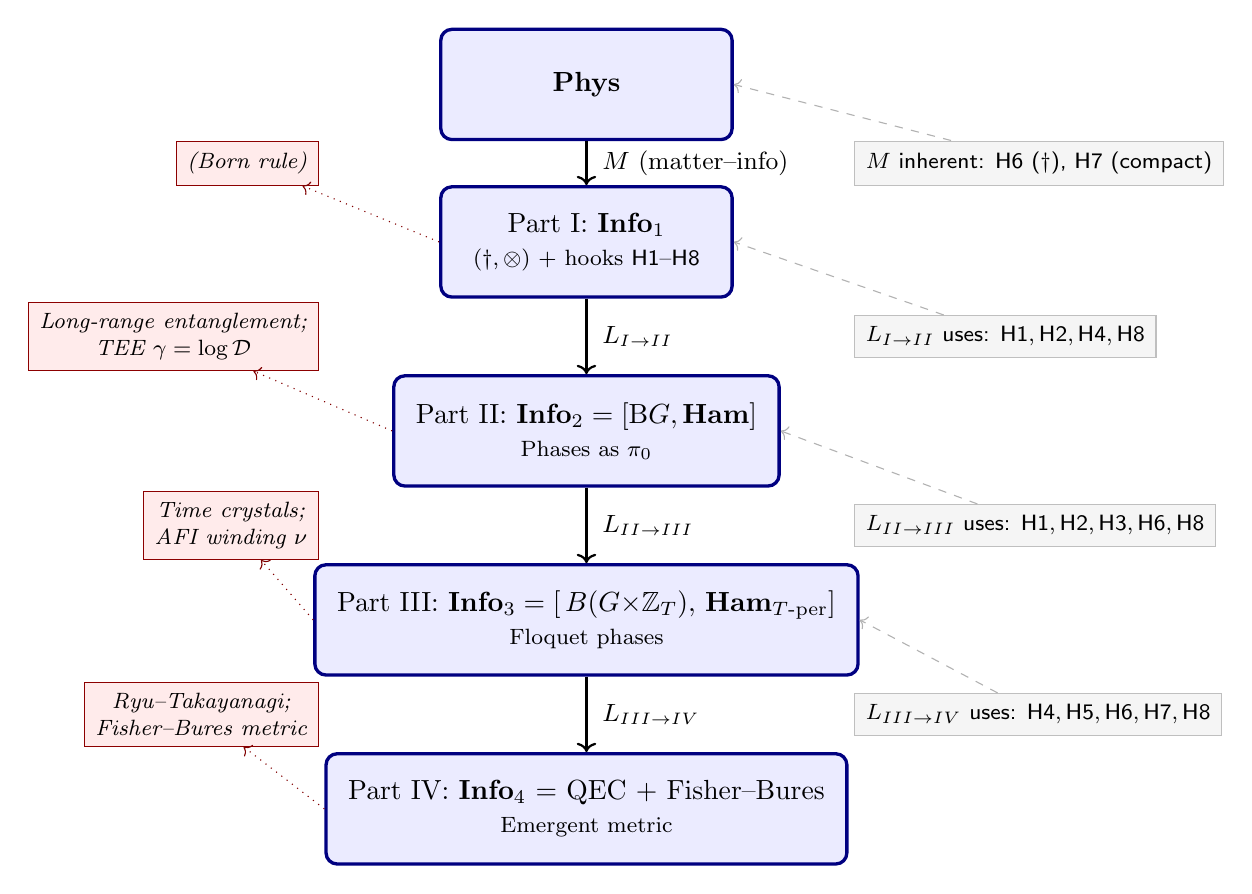
\begin{tikzpicture}[
  node distance=11mm and 22mm,
  every node/.style={align=center},
  layer/.style={
    rectangle, rounded corners, draw=blue!50!black, very thick,
    fill=blue!8, inner sep=8pt, minimum width=37mm, minimum height=14mm
  },
  hooks/.style={
    rectangle, draw=gray!50, fill=gray!8, inner sep=4pt,
    font=\footnotesize\sffamily
  },
  emerg/.style={
    rectangle, draw=red!55!black, fill=red!8, inner sep=4pt,
    font=\footnotesize\itshape
  }
]
\node[layer] (P)  at (0, 0)        {$\Phys$};
\node[layer] (I1) at (0, -2.0)     {Part I: $\Info_1$\\\footnotesize$(\dagger,\otimes)$ + hooks $\mathsf{H1}$--$\mathsf{H8}$};
\node[layer] (I2) at (0, -4.4)     {Part II: $\Info_2 = [\BG,\Ham]$\\\footnotesize Phases as $\pi_0$};
\node[layer] (I3) at (0, -6.8)     {Part III: $\Info_3 = [\,B(G{\times}\Z_T),\,\Ham_{T\text{-per}}]$\\\footnotesize Floquet phases};
\node[layer] (I4) at (0, -9.2)     {Part IV: $\Info_4$ = QEC + Fisher--Bures\\\footnotesize Emergent metric};

\draw[->, thick] (P) -- node[right=2pt, font=\small]{$M$ (matter--info)} (I1);
\draw[->, thick] (I1) -- node[right=2pt, font=\small]{$L_{I\to II}$} (I2);
\draw[->, thick] (I2) -- node[right=2pt, font=\small]{$L_{II\to III}$} (I3);
\draw[->, thick] (I3) -- node[right=2pt, font=\small]{$L_{III\to IV}$} (I4);

\node[hooks, anchor=west] (h1) at (3.4, -1.0)  {$M$ inherent: $\mathsf{H6}$ ($\dagger$), $\mathsf{H7}$ (compact)};
\node[hooks, anchor=west] (h2) at (3.4, -3.2)  {$L_{I\to II}$ uses: $\mathsf{H1}, \mathsf{H2}, \mathsf{H4}, \mathsf{H8}$};
\node[hooks, anchor=west] (h3) at (3.4, -5.6)  {$L_{II\to III}$ uses: $\mathsf{H1}, \mathsf{H2}, \mathsf{H3}, \mathsf{H6}, \mathsf{H8}$};
\node[hooks, anchor=west] (h4) at (3.4, -8.0)  {$L_{III\to IV}$ uses: $\mathsf{H4}, \mathsf{H5}, \mathsf{H6}, \mathsf{H7}, \mathsf{H8}$};

\draw[->, gray!60, dashed] (h1) -- (P.east);
\draw[->, gray!60, dashed] (h2) -- (I1.east);
\draw[->, gray!60, dashed] (h3) -- (I2.east);
\draw[->, gray!60, dashed] (h4) -- (I3.east);

\node[emerg, anchor=east] (e1) at (-3.4, -1.0) {(Born rule)};
\node[emerg, anchor=east] (e2) at (-3.4, -3.2) {Long-range entanglement;\\ TEE $\gamma=\log\mathcal{D}$};
\node[emerg, anchor=east] (e3) at (-3.4, -5.6) {Time crystals;\\ AFI winding $\nu$};
\node[emerg, anchor=east] (e4) at (-3.4, -8.0) {Ryu--Takayanagi;\\ Fisher--Bures metric};

\draw[->, red!50!black, dotted] (I1.west) -- (e1);
\draw[->, red!50!black, dotted] (I2.west) -- (e2);
\draw[->, red!50!black, dotted] (I3.west) -- (e3);
\draw[->, red!50!black, dotted] (I4.west) -- (e4);
\end{tikzpicture}
\caption{Compositional functor chain of the four-paper series. Solid
arrows are $1$-cells in $\Theory$ (functorial liftings). Dashed gray
arrows show which hooks are consumed by each lift, as detailed in the
ledger (\Cref{sec:hook-ledger}). Dotted red arrows indicate emergent
properties produced at each layer. The diagram is hierarchical: each
layer plugs into the typed slots declared by its predecessors and
exposes new typed slots for its successors.}
\label{fig:main-diagram}
\end{figure}

\subsection{Coherence of the composition}

\begin{theorem}[Composition is well-typed]
\label{thm:composition}
Within $\Theory$, the composition
\[
L := L_{III \to IV} \circ L_{II \to III} \circ L_{I \to II} \circ M : \Phys
\to \Info_4
\]
is a well-defined $1$-cell. In particular, every hook consumed by an
intermediate lift is supplied by a strictly earlier layer; no hook is left
unfilled.
\end{theorem}

\begin{proof}[Proof sketch]
By the hook ledger of \Cref{sec:hook-ledger}, each lift consumes only
Part~I-declared hooks $\mathsf{H1}$--$\mathsf{H8}$ together with the
forward-pointing hooks declared by its strict predecessor (the five
Part~II hooks for $L_{II\to III}$; the four Part~III hooks for
$L_{III\to IV}$). Hooks $\mathsf{H6}$ and $\mathsf{H7}$ are inherent to
$M$ (dagger and compact-closure preservation) and are inherited by every
downstream layer, so the lifts are free to consume them where needed.
Composition of $1$-cells in $\Theory$ requires hook-respecting strong
monoidal $\dagger$-functors; each constituent $L_{i\to i+1}$ is so by
Part~II Proposition 2.14 ($L_{I\to II}$), Part~III Proposition 4.6
($L_{II\to III}$), and Part~IV Remark 8.1 ($L_{III\to IV}$). Composition
is associative by the functoriality of all constituents, and the
identity $1$-cells are preserved.
\end{proof}

\begin{remark}[Rigour gradient and its implications]
\label{rem:limit-rigour}
\Cref{thm:composition} is a structural assertion about the typed signature
of the composition. It is \emph{not} a statement that the highest-level
emergent claims (e.g.\ that the Fisher--Bures metric on a CFT state space
agrees with the bulk AdS metric) are theorems. The rigour profile is
layered:
\begin{itemize}[leftmargin=2em]
\item $L_{I \to II}$ is mathematically rigorous: the SPT classification by
  $H^{d+1}(G, U(1))$ \cite{chen2013}, the MTC classification of $(2{+}1)$D
  topological phases \cite{kitaev2003, levinwen2005}, and the
  Kitaev--Preskill--Levin--Wen formula for $\gamma$ \cite{kitaevpreskill2006}
  are provably correct.
\item $L_{II \to III}$ is rigorous in the prethermal regime $t \leq \tau_*
  \sim \exp(c\,\omega/J)$ and for MBL-protected DTCs \cite{else2016,
  bukov2015}, but breaks down in the heating regime where it currently
  lacks a categorical formulation.
\item $L_{III \to IV}$ is rigorous in the discrete HaPPY model
  \cite{pyhp2015} (where the Ryu--Takayanagi formula is exact) and in the
  semiclassical limit of continuum holography \cite{ryutakayanagi2006,
  fghmv2014}, but the full non-perturbative continuum statement
  (Miyaji--Takayanagi conjecture \cite{miyajitakayanagi2015}) remains
  open.
\end{itemize}
This gradient has three concrete implications. (1)~\emph{Testability is
layered}\/: the modular thesis is empirically testable at the lower layers
(SPT phases observed in cold-atom and topological-insulator experiments;
DTCs observed in trapped-ion arrays \cite{zhang2017}; HaPPY-style codes
implementable on near-term NISQ devices) and currently structural at the
highest layer (continuum holographic claims). (2)~\emph{Verifiability of
non-derivability}: \Cref{prop:gen-nonderiv} is provably tight at the
discrete level (where Part~IV exhibits explicit counterexamples), and
remains a structural assertion at the continuum level. (3)~\emph{Robustness
of the modular thesis}: even in the conjectural regime, the modular thesis
is well-typed (\Cref{thm:composition}); refining the conjectural lifts to
theorems is a research programme, not a pre-condition for the framework's
utility. Part~IV is explicit about this gradient and presents its
constituent results layer by layer.
\end{remark}

\subsection{The composite as a $1$-cell, and Proposition 8.2 generalised}

The composite $L : \Phys \to \Info_4$ produces an emergent geometry from a
quantum-information substrate. The non-derivability content is:

\begin{proposition}[Generalised non-derivability]
\label{prop:gen-nonderiv}
For each strict subset $S \subsetneq \{I, II, III, IV\}$, there exists a
filling of the hooks of $\bigcup_{i \in S} \mathrm{Part}_i$ that produces
no element of $\Info_4$ exhibiting the Fisher--Bures Riemannian metric of
Part~IV. Equivalently, the composite $L$ is not factorable through any
proper sub-chain of \eqref{eq:main-chain}.
\end{proposition}

\begin{proof}[Proof sketch]
The case $S = \{I, II, III\}$ is precisely Proposition 8.2 of Part~IV, whose
proof exhibits explicit counterexamples in $\FHilb$, in the toric code, and
in any Floquet system on a Hilbert space without long-range entanglement.
For smaller subsets $S$, the same counterexamples apply: an example showing
non-derivability from $\{I, II, III\}$ a fortiori shows non-derivability
from any proper subset.
\end{proof}

\Cref{prop:gen-nonderiv} is the precise modular thesis: \emph{emergent
geometry is irreducibly compositional}.

\section{Cross-cutting Themes}
\label{sec:themes}

We now isolate six themes that thread all four constituent papers. Each is a
quantitative or structural through-line whose appearance in multiple layers
illuminates the compositional architecture.

\subsection{Theme 1: entanglement entropy as quantitative through-line}
\label{sec:theme-EE}

\begin{theme}[Entanglement entropy across layers]
\label{theme:EE}
The von Neumann entropy $S(A) = -\Tr(\rho_A \log \rho_A)$ appears, with
distinct quantitative content, at every layer of the framework:
\begin{itemize}[leftmargin=2em]
\item In Part~I, $S$ is the trace $\Tr$ in a compact closed dagger
  category, applied to the matter--information image of a reduced density
  matrix.
\item In Part~II, the topological entanglement entropy $\gamma = \log
  \mathcal{D}$ is a phase invariant; $S(A) = \alpha |\partial A| - \gamma +
  O(1/|A|)$ on a disk.
\item In Part~III, the Floquet TEE $\gamma_T = \log \mathcal{D}_T$ is a
  Floquet phase invariant on the Floquet enriched MTC $\mathcal{C}_T =
  \mathcal{C} \boxtimes \Rep(\Z_T)$.
\item In Part~IV, the Ryu--Takayanagi formula $S(A) = \Area(\gamma_A) /
  (4G_N)$ identifies entanglement entropy with the area of a bulk minimal
  surface; in the discrete HaPPY model this is exact.
\end{itemize}
\end{theme}

The progression is hierarchical. Part~I gives the categorical type of $S$:
it is a functor $\mathbf{Reg}^\op \to \R_{\geq 0}$ defined as
$S(A) = -\Tr(\rho_A \log \rho_A)$, where $\Tr$ is the trace of the compact
closed dagger structure of $\Phys$ and $\rho_A$ is obtained by partial trace
along $\eta, \varepsilon$. Part~II gives a topological constant $\gamma$
that detects long-range entanglement. Part~III decorates this with a
temporal index. Part~IV identifies $S$ with a geometric area. The same
quantitative object acquires new meanings as we ascend.

\subsection{Theme 2: symmetry-protected structure}
\label{sec:theme-SPT}

\begin{theme}[Symmetry across layers]
\label{theme:SPT}
The role of symmetry refines as the framework composes:
\begin{itemize}[leftmargin=2em]
\item In Part~I, hook $\mathsf{H1}$ specifies a $G$-action $\rho :
  B\mathcal{G} \to \mathrm{Aut}(\Phys)$.
\item In Part~II, this action classifies SPT phases by $H^{d+1}(G, U(1))$
  (Chen--Gu--Liu--Wen), with the classification refining to a functor
  $\mathrm{SPT}^d : \mathbf{Grp} \to \mathbf{Ab}$.
\item In Part~III, the symmetry enlarges by $\Z_T$ (discrete temporal
  translation); the relevant cohomology becomes $H^{d+2}(G \times \Z_T,
  U(1))$.
\item In Part~IV, the symmetry of the boundary CFT and its modular flow
  generate the bulk emergent diffeomorphism symmetry; the modular flow is
  Tomita--Takesaki theory restricted to half-spaces in the vacuum.
\end{itemize}
\end{theme}

The pattern: a symmetry that is local in Part~I becomes a classification
parameter in Part~II, gains a temporal factor in Part~III, and is finally
identified with a geometric symmetry in Part~IV. This progression --- from
algebraic to geometric symmetry --- directly underlies emergent properties
\Cref{em:lre,em:tee,em:dtc,em:happy} of \Cref{sec:catalogue}.

\subsection{Theme 3: fixed-point reasoning}
\label{sec:theme-fp}

\begin{theme}[Fixed points across layers]
\label{theme:fp}
Each layer involves a critical fixed-point construction:
\begin{itemize}[leftmargin=2em]
\item Part~I: Mac Lane coherence (every well-typed diagram commutes) is a
  strict-monoidal fixed-point statement.
\item Part~II: Renormalisation-group fixed points represent each phase
  $[H] \in \pi_0(\Ham)$; an RG flow $H \to H'$ converges to a fixed point
  of the coarsening functor.
\item Part~III: Magnus fixed points --- the prethermal effective
  Hamiltonian is the limit of the Magnus colimit on a finite truncation;
  Floquet stationary states are fixed points of $U(T)$.
\item Part~IV: HaPPY tensor-network fixed points are the bulk holographic
  states; the Bures metric is the unique monotone metric (Chentsov fixed
  point).
\end{itemize}
\end{theme}

In every case the fixed-point structure is what makes the categorical
content into a phase invariant. The dictionary fixed-point $\leftrightarrow$ phase
representative is constant across layers.

\subsection{Theme 4: functorial pullback}
\label{sec:theme-pullback}

\begin{theme}[Pullback of structure]
\label{theme:pullback}
The composition mechanism is functorial pullback:
\begin{itemize}[leftmargin=2em]
\item Part~II's classification of $G$-symmetric phases is the connected
  components of the functor category $[\BG, \Ham_0]^{\mathrm{eq}}$,
  obtained as pullback of the trivial $\BG$-functor along $\rho$.
\item Part~III's Floquet enrichment is the pullback of the equilibrium
  phase functor along the inclusion $B\Z_T \hookrightarrow B(G \times
  \Z_T)$, intersected with the prethermal regime.
\item Part~IV's bulk-to-boundary functor is the pullback of the global
  state along the inclusion of a boundary region, mediated by the QEC
  encoder.
\end{itemize}
\end{theme}

Pullback is the universal way to ``restrict'' a structure along an
inclusion or projection, and it is what makes our composition a categorical
operation rather than ad-hoc gluing.

\subsection{Theme 5: dagger preservation}
\label{sec:theme-dagger}

\begin{theme}[$\dagger$ across layers]
\label{theme:dagger}
The $\dagger$-structure of Part~I is preserved by every subsequent lift:
\begin{itemize}[leftmargin=2em]
\item Part~II requires unitary representations of $G$, so the
  symmetry-action functor is $\dagger$-preserving.
\item Part~III's Floquet evolution is by definition unitary; the Floquet
  functor lands in $\mathbf{Unit} \subset \QChan$ (a $\dagger$-monoidal
  subcategory).
\item Part~IV's QEC encoder is a $\dagger$-isometry; complementary recovery
  is the assertion that recovery is a $\dagger$-section of the encoder.
\end{itemize}
\end{theme}

Consequently the matter--information functor's dagger-preservation
property propagates up the chain: every emergent piece of structure inherits
unitarity. This is the categorical reason why Floquet drives are unitary
and why holographic codes are isometries.

\subsection{Theme 6: obstruction $2$-cells}
\label{sec:theme-obstruction}

\begin{theme}[Obstructions detect emergent phenomena]
\label{theme:obstr}
At each compositional layer, novel phenomena are detected as obstruction
$2$-cells:
\begin{itemize}[leftmargin=2em]
\item Part~II: phase transitions are non-invertible natural transformations
  $\eta : F \Rightarrow F'$ between gapped Hamiltonian functors (the
  ``obstruction'' is the gap closing).
\item Part~III: discrete time crystals are obstruction $2$-cells in the
  comparison between iterated and re-labelled Floquet drives; Floquet
  winding numbers are obstructions to homotopies of Floquet--Bloch
  functors.
\item Part~IV: the AMPS firewall paradox is an obstruction to monogamy of
  entanglement under naive locality; OAQEC complementary recovery resolves
  it by replacing local bulk operators with non-local boundary
  reconstructions.
\end{itemize}
\end{theme}

The categorical reading: every phenomenon ``without an equilibrium analog'' or
``not derivable from local data'' is an obstruction class in the appropriate
$2$-categorical structure.

\section{Emergent Property Catalogue}
\label{sec:catalogue}

We now catalogue twelve emergent properties of the modular framework. Each
is labelled with the lowest law-level at which it appears and accompanied
by a proof sketch that it is non-derivable from any subset of strictly
fewer laws. The catalogue generalises Proposition 8.2 of Part~IV.

\paragraph{Selection criterion.}
The twelve properties are selected to satisfy three criteria: (i) each is
identified as a principal mathematical or physical contribution of one of
the constituent papers; (ii) each admits an explicit non-derivability
witness exhibitable from the worked examples of the constituent papers;
and (iii) collectively they cover all four constituent papers, with at
least two properties per Part. Properties that are technically interesting
but reducible to a strict sub-chain (e.g.\ specific anyon braiding rules,
which already appear at Part~II's MTC level without needing Part~I's
operadic data) are not included.

\paragraph{Connection to cross-cutting themes.}
Each of the six cross-cutting themes of \Cref{sec:themes} appears
concretely in the catalogue:
\begin{itemize}[leftmargin=2em]
\item \Cref{theme:EE} (entanglement entropy) underlies
  \Cref{em:tee,em:rt} via $\gamma$ and the area formula;
\item \Cref{theme:SPT} (symmetry) underlies \Cref{em:dtc,em:afi};
\item \Cref{theme:fp} (fixed points) underlies \Cref{em:preth,em:fisher};
\item \Cref{theme:pullback} (functorial pullback) underlies
  \Cref{em:lre,em:happy};
\item \Cref{theme:dagger} (dagger) underlies \Cref{em:smc,em:born,em:qec};
\item \Cref{theme:obstr} (obstruction $2$-cells) underlies
  \Cref{em:dtc,em:afi}.
\end{itemize}
Thus the themes are not parallel observations but unifying mechanisms: each
theme produces concrete emergent properties, and the modular thesis
asserts that all themes simultaneously hold along the composite $L$.

\subsection{Layer-by-layer enumeration}

\begin{emerg}[Strong-monoidal $\dagger$-structure]
\label{em:smc}
\textbf{Layer:} Part~I. The category $\Phys$ admits a $\dagger$-symmetric
monoidal compact closed structure (Theorem 2.7 of Part~I). \textbf{Proof of
non-derivability:} no smaller axiomatic system can simultaneously accommodate
both quantum (no-cloning, demanding non-cartesian tensor) and topological
(compact closure, demanding duals) structure. A purely cartesian category
admits diagonals and thus violates no-cloning.
\end{emerg}

\begin{emerg}[Born-rule formula]
\label{em:born}
\textbf{Layer:} Part~I. The probability formula $p(\phi | \psi) =
|\langle \phi | \psi \rangle|^2$ arises as a categorical theorem from
compact-closure plus dagger (Theorem 3.5 of Part~I).
\textbf{Non-derivability:} the formula is built from the trace of a
composite morphism $\varepsilon \circ (\phi^\dagger \otimes \id) \circ
\eta \circ \psi : I \to I$. Without compact closure (hook
$\mathsf{H7}$), the unit $\eta$ and counit $\varepsilon$ are absent and
the trace is undefined; without dagger (hook $\mathsf{H6}$), the
adjoint $\phi^\dagger$ is undefined and the formula's symmetric form
$|\langle\phi|\psi\rangle|^2 = \langle\phi|\psi\rangle\langle\psi|\phi\rangle$
cannot be assembled. Both ingredients are inherent to $M$, so the
property emerges at Part~I and not before.
\end{emerg}

\begin{emerg}[Long-range entanglement]
\label{em:lre}
\textbf{Layer:} Part~II. There exist gapped ground states (e.g.\ toric code)
that cannot be transformed into a product state by any finite-depth local
quantum circuit. \textbf{Non-derivability from Part~I alone:} Part~I's
categorical machinery does not specify a notion of locality without the
sheaf hook $\mathsf{H4}$; with $\mathsf{H4}$ but without a designated
sub-category $\Ham$ (hook $\mathsf{H2}$), the connected-component invariant
$\pi_0(\Ham)$ is undefined.
\end{emerg}

\begin{emerg}[Topological entanglement entropy $\gamma = \log \mathcal{D}$]
\label{em:tee}
\textbf{Layer:} Part~II. For a topologically ordered phase, $S(A) = \alpha
|\partial A| - \gamma$ on a disk $A$, with $\gamma = \log \mathcal{D}$
universal. \textbf{Non-derivability:} requires both Part~I (compact closure
to define traces, hence entropy) and Part~II (modular tensor category data
giving $\mathcal{D}$). Neither alone produces a numerical phase invariant.
\end{emerg}

\begin{emerg}[Anyonic statistics]
\label{em:anyon}
\textbf{Layer:} Part~II. Quasi-particles in $(2{+}1)$D topological phases obey
braided fusion rules with non-trivial topological spin $\theta_a = e^{2\pi i
h_a}$. \textbf{Non-derivability:} requires the modular tensor category data
of Part~II. Part~I alone gives only symmetric (boson/fermion) statistics; the
truly braided structure is a Part~II emergent feature.
\end{emerg}

\begin{emerg}[Discrete time crystals (DTCs)]
\label{em:dtc}
\textbf{Layer:} Part~III. There exists a Floquet phase whose stroboscopic
order parameter oscillates with period $2T$ (twice the drive period) for all
times in the thermodynamic limit (Else--Bauer--Nayak 2016).
\textbf{Non-derivability:} requires Part~I (categorical formulation),
Part~II (spontaneous symmetry breaking machinery), \emph{and} Part~III
(Floquet hook $\mathsf{H3}$ supplying $B\Z_T$). Watanabe--Oshikawa~\cite{watanabe2015} show DTCs
are forbidden in equilibrium; they emerge only when the Floquet temporal
structure is added.
\end{emerg}

\begin{emerg}[Anomalous Floquet topological insulators (AFI)]
\label{em:afi}
\textbf{Layer:} Part~III. The $\nu = 1$ AFI phase has chiral edge modes at
quasi-energy $\pi$ with all bulk Chern numbers vanishing.
\textbf{Non-derivability:} the bulk Chern number is a Part~II equilibrium
invariant; the AFI exists \emph{only} when this invariant vanishes, so AFI is
not a Part~II phenomenon. It is detected by the Floquet winding number
$\nu = \frac{1}{24\pi^2} \int \Tr[(U^\dagger dU)^3]$, which requires the
Part~III spatio-temporal Brillouin torus $\mathrm{BZ} \times S^1$.
\end{emerg}

\begin{emerg}[Prethermal phases]
\label{em:preth}
\textbf{Layer:} Part~III. For drive frequency $\omega \gg J$, the system is
governed by a prethermal effective Hamiltonian for time $t \leq \tau_* \sim
\exp(c \omega/J)$. \textbf{Non-derivability:} requires the Magnus expansion
(Part~III) and the equilibrium phase classifier of Part~II to interpret
$H_{\mathrm{eff}}$ as a Part~II phase; neither alone produces the prethermal
correspondence.
\end{emerg}

\begin{emerg}[Quantum error-correcting code structure of long-range
  entanglement]
\label{em:qec}
\textbf{Layer:} Part~IV (using Part~II). Topologically ordered phases are
quantum error-correcting codes (Bombin--Mart\'{\i}n-Delgado 2006; Kitaev 2003).
\textbf{Non-derivability from Part~II alone:} Part~II classifies the phase but
does not exhibit it as a code without the Part~I dagger structure
(hook $\mathsf{H6}$) and the Part~IV operator-algebra QEC formalism.
\end{emerg}

\begin{emerg}[Holographic isometry]
\label{em:happy}
\textbf{Layer:} Part~IV. The HaPPY tensor network defines an isometric
embedding $V : \Hilb_{\mathrm{bulk}} \to \Hilb_{\mathrm{boundary}}$.
\textbf{Non-derivability:} requires Part~I (string-diagram/tensor-network
calculus), Part~II (long-range entanglement as the substrate), \emph{and}
Part~IV's perfect-tensor construction. The construction is constructive only
when all three are composed.
\end{emerg}

\begin{emerg}[Ryu--Takayanagi area formula]
\label{em:rt}
\textbf{Layer:} Part~IV. $S(A) = \Area(\gamma_A) / (4G_N)$ exact in the
HaPPY model~\cite{pyhp2015,harlow2017}. \textbf{Non-derivability:} this is
exactly Proposition 8.2 of Part~IV. We exhibit (i) $\FHilb$ models satisfying all of Part~I but
producing no area law; (ii) Part~II models (toric code) producing $\gamma
= \log \mathcal{D}$ but no area-of-a-surface formula; (iii) Part~III models
(generic Floquet on a non-LRE Hilbert space) producing modular flow but no
area law. Only the composite $L$ produces an RT formula.
\end{emerg}

\begin{emerg}[Fisher--Bures Riemannian metric on parametric state
  manifolds]
\label{em:fisher}
\textbf{Layer:} Part~IV. Each parametric family $\{\rho_\theta\}$ acquires a
canonical Riemannian metric $g_{ij}^Q$ from Chentsov monotonicity.
\textbf{Non-derivability:} the symmetric logarithmic derivative $L_i$
requires a smooth parametric dependence (Part~III input via the Floquet
parametric family) plus a long-range entangled substrate (Part~II input)
plus the categorical $\dagger$-structure (Part~I hook $\mathsf{H6}$).
\end{emerg}

\subsection{Tabular summary}

\begin{center}
\small
\renewcommand{\arraystretch}{1.18}
\begin{tabular}{@{}rlll@{}}
\toprule
\# & Property & Layer & Non-derivability witness \\
\midrule
1 & $\dagger$-symmetric monoidal structure       & I       & cartesian categories \\
2 & Born rule                                    & I       & non-compact-closed cat. \\
3 & Long-range entanglement                      & II      & $\FHilb$ alone \\
4 & TEE $\gamma = \log \mathcal{D}$              & II      & SRE phases \\
5 & Anyonic statistics                           & II      & symmetric MC alone \\
6 & Discrete time crystals                       & III     & equilibrium SSB \\
7 & AFI winding number                           & III     & equilibrium Chern bands \\
8 & Prethermal phases                            & III     & static $H$ alone \\
9 & QEC structure of LRE                         & II + IV & Part~II w/o $\dagger$ \\
10 & Holographic isometry $V$                    & IV      & Part~I alone (no LRE) \\
11 & Ryu--Takayanagi area formula                & IV      & Part~III w/o LRE \\
12 & Fisher--Bures metric                        & IV      & Any proper subset of \{I, II, III\} alone \\
\bottomrule
\end{tabular}
\end{center}

\subsection{Compositional structure of the catalogue}

The catalogue exhibits the modular thesis empirically: of twelve listed
emergent properties, five appear at Part~III or Part~IV (where the highest
compositional content is required), and these five are precisely those
associated with novel non-equilibrium or geometric phenomena (DTCs, AFI,
prethermal, holographic isometry, RT formula, Fisher--Bures metric). The
remaining seven appear at Parts I or II and are correspondingly more
``algebraic''.

The non-derivability witnesses follow a uniform pattern: for each property,
we exhibit an explicit object satisfying \emph{some} subset of the prior
laws but \emph{not} the property in question. The pattern works because the
modular framework is genuinely typed: each layer adds qualitatively new
typed slots, and absent any layer, the corresponding slot is empty.

\section{Open Compositional Problems}
\label{sec:open}

We close with eleven open problems organised by layer. Each is either a
formalisation gap (a missing theorem in the modular composition itself) or a
testable prediction (a physical question whose answer would constrain the
framework).

\subsection*{Problems on the lifts themselves}

\begin{enumerate}[label=O\arabic*., leftmargin=2.6em]

\item \emph{Categorification of the $2$-category $\Theory$.}
Refine \Cref{def:theory} to a homotopy-coherent $(\infty,2)$-category of
physical theories accommodating gauge symmetries as $\infty$-groupoids.
Determine whether the chain \eqref{eq:main-chain} extends to a full
$(\infty, 2)$-functor.

\item \emph{Rigorous Floquet--Floquet composition.}
The lift $L_{II \to III}$ is rigorous in the prethermal regime (time $t
\leq \tau_*$) and for MBL-protected DTCs. Outside these regimes, what is the
correct categorical statement of Floquet phase classification when the
system heats to infinite temperature? Is there a colimit-completion of the
prethermal lift that captures the heating regime?

\item \emph{Categorical AdS/CFT.}
Formulate the AdS/CFT duality as a precise functor between well-defined
$\infty$-categories. The functor should restrict to the HaPPY isometry on
the discrete tiling and to the Maldacena duality on its semiclassical limit.
This is open at the level of both the source and the target categories.

\item \emph{Non-perturbative Ryu--Takayanagi.}
The HaPPY model exhibits an exact RT formula. The semiclassical RT formula
\cite{ryutakayanagi2006} is rigorous to leading order in $G_N$. Is there a
non-perturbative compositional derivation interpolating these two regimes
(perhaps via the island formula and the quantum extremal surface
prescription)?

\end{enumerate}

\subsection*{Problems involving cross-cutting themes}

\begin{enumerate}[label=O\arabic*., leftmargin=2.6em, resume]

\item \emph{Floquet holography.}
What is the holographic dual of a Floquet CFT on the boundary? Does the
bulk become time-dependent in a controlled way (perhaps a slowly-rotating
geometry in the prethermal regime)? The Part~III hooks for Part~IV imply
that DTC obstruction $2$-cells should correspond to non-trivial
$2$-morphisms in the holographic functor; explicit examples are absent.

\item \emph{Categorical fracton order.}
Fracton phases~\cite{vijayhaahfu2016} have sub-extensive ground-state
degeneracy and sub-system symmetries, neither of which fits in the
modular tensor category framework of Part~II. Find a categorical
extension of the Part~II classification (perhaps via higher categories,
or via fusion $2$-categories) that captures fractons. This bears
directly on the modular composition since fracton phases composed with
Part~III drives produce ``fracton time crystals'' whose existence is
empirically suggested but unclassified.

\item \emph{Fisher metric = bulk metric (Miyaji--Takayanagi).}
The Miyaji--Takayanagi conjecture asserts that the Fisher--Bures metric on
the space of CFT states equals the bulk AdS metric. Prove or disprove
this in a controlled limit (e.g.\ large-$N$, large-coupling, on a fixed
state space). A modular formulation: the conjecture asserts that the
emergent metric functor of Part~IV factors through a continuum limit.

\item \emph{Continuous time crystals.}
The Watanabe--Oshikawa no-go theorem~\cite{watanabe2015} precludes continuous time-crystalline
phases in equilibrium. Is there a Part~III + Part~IV framework in which
\emph{quasi-continuous} time-translation symmetry breaking arises from
holographic codes whose boundary CFTs flow under irrational
modular periods?

\end{enumerate}

\subsection*{Problems on the modular thesis}

\begin{enumerate}[label=O\arabic*., leftmargin=2.6em, resume]

\item \emph{Tightness of the non-derivability proposition.}
\Cref{prop:gen-nonderiv} (and Proposition 8.2 of Part~IV) is
non-derivability \emph{within the proposed schema}. Is there a stronger
statement: that no alternative compositional framework with strictly
fewer ingredients can reproduce the Fisher--Bures metric? This is open at
the level of formalisation.

\item \emph{Operational signature of compositionality.}
The modular thesis claims emergent properties arise only from composition.
Operationally, can we design an experiment (e.g.\ a quantum simulator
with Floquet drive on a topologically ordered substrate) whose output is
provably accessible only when all three of Parts II--III--IV's
ingredients are present? A positive answer would convert the modular
thesis from a structural to a genuinely empirical claim.

\item \emph{Comparison with alternative compositional schemes.}
The Schreiber--Shulman cohesive HoTT framework~\cite{schreibershulman2014},
the Costello--Gwilliam factorisation algebra framework~\cite{costello2017},
and the algebraic QFT of Haag--Kastler each provide alternative
compositional formalisms. Establish precise
comparison functors between these and our $\Theory$. The comparison
should address (a) categorical primitives (which monoidal/$\dagger$/2-categorical
data each framework axiomatises); (b) compositional rules (how each
framework builds layered constructions); (c) scope of emergent phenomena
captured (which of \Cref{em:smc}--\ref{em:fisher} each framework reaches).
Are any of them isomorphic at the Part~I level? At the Part~I + Part~II
level? What about higher levels?

\end{enumerate}

\section{Conclusion and Outlook}
\label{sec:conclusion}

\subsection{Summary}

We have presented the synthesis of a four-paper modular research series on
emergent spacetime dynamics. The central thesis is that the emergent
properties of physical structure --- from long-range entanglement and
anyonic statistics, through time crystals and anomalous Floquet
invariants, to the Ryu--Takayanagi area formula and the Fisher--Bures
metric --- are \emph{compositional}\/: each emerges from the layered
combination of prior categorical structures via explicit functorial
liftings, not from any single law in isolation. We have:

\begin{itemize}[leftmargin=2em]
\item recapped the categorical primitives contributed by each constituent
  paper (\Cref{sec:recap});
\item tabulated the eight Composition Hooks of Part~I and their
  consumption sites across Parts II--IV (\Cref{sec:hook-ledger});
\item presented the compositional functor chain $\Phys \to \Info_1 \to
  \Info_2 \to \Info_3 \to \Info_4$ as a $1$-cell in a $2$-category
  $\Theory$ of physical theories, with explicit hook tracking
  (\Cref{sec:functor-chain});
\item isolated six cross-cutting themes that thread all four papers
  (\Cref{sec:themes});
\item catalogued twelve emergent properties with non-derivability
  witnesses, generalising Proposition 8.2 of Part~IV
  (\Cref{sec:catalogue});
\item enumerated eleven open compositional problems, with explicit
  formalisation gaps and testable predictions (\Cref{sec:open}).
\end{itemize}

\subsection{Modular composition is the mechanism}

The slogan of the series is that \emph{modular composition is the mechanism}.
This means three interrelated things. First, the framework is not a
unification: replacing any single layer with a different filling of its hook
leaves the remainder intact. Second, the framework is genuinely typed: each
hook has a categorical signature that any candidate filling must respect.
Third, the emergent content of the framework is irreducibly compositional:
no proper sub-chain produces the highest-level outputs.

Taken together these three commitments make the modular framework an
engineering discipline as much as a mathematical one. New physical theories
can be slotted in as alternative fillings of any hook; the rest of the
framework continues to apply, with appropriate updates to the typed outputs.
The synthesis is thus an interface specification, not a closed system.

\subsection{Outlook: extensions and applications}

We close with six speculative directions for extending the modular
framework, ordered roughly by ambition.

\begin{enumerate}[label=\arabic*., leftmargin=2.4em]
\item \emph{de Sitter holography.} The framework is articulated for
AdS-style holography (Part~IV). Replace the hyperbolic tiling by a
spherical or de Sitter analog and ask whether the modular composition
produces a dS bulk. The answer is presumably Part-IV-specific (the
modular composition up to Part~III is geometry-agnostic), but the
precise formulation is open.

\item \emph{Quantum simulators.} The Haskell encodings in each paper
are designed for executable verification on small instances. A natural
extension is to a programmable quantum simulator (e.g.\ a NISQ device)
that realises the Part~IV holographic code on a Floquet-driven Part~II
substrate, validating the compositional thesis at experimental scale.

\item \emph{Fault-tolerant computation.} Part~II topological order is
the substrate of fault-tolerant quantum computation. The Part~III
Floquet extension produces drive-stabilised codes whose error rates
scale with $\exp(c \omega / J)$ in the prethermal regime. The Part~IV
holographic extension might reveal that fault tolerance is itself an
emergent geometric property.

\item \emph{Categorical machine learning.} The Fisher--Bures metric of
Part~IV is the natural geometry of statistical inference. Extending the
modular framework to encompass classical statistical learning (where
Part~II is replaced by a classification of statistical phases) is a
direction with applications to machine-learning theory.

\item \emph{Higher-categorical refinements.} Each layer can be refined
to higher-categorical analogues: $(2,2)$-categorical Part~I for
extended TQFTs, fusion $2$-categories for Part~II $(3{+}1)$D
topological phases, etc. The modular composition should extend
coherently; verifying this is open work.

\item \emph{Quantum gravity.} The most ambitious extension: identify
the modular framework's Part~IV outputs with the elementary quanta of
quantum gravity. The Fisher--Bures metric then becomes a candidate for
the quantum gravitational metric, and emergent diffeomorphism
invariance is a Part-IV emergent symmetry. Whether this can be made
precise is the single largest open problem of the series.
\end{enumerate}

\subsection{Final remarks}

We end where we began. The four-paper series \emph{Emergent Spacetime
Dynamics} is a modular framework, not a unified theory. Its claims are
structural: that emergent geometry can be \emph{built}, not merely
\emph{posited}, by the compositional layering of categorical, phase,
modulation, and information-geometric structure. The synthesis is the
articulation of how this building proceeds: which hooks are consumed at
each layer, which emergent properties appear at each layer, and which are
irreducibly compositional. We hope it provides a usable framework for
further work --- both critical (challenging individual lifts or hooks) and
constructive (proposing alternative fillings) --- rather than a closed
edifice. The conviction that motivated us throughout was that physics
composes, that composition is itself a mathematical operation, and that
spacetime is one of its emergent outputs.

\section*{Acknowledgements}

The authors thank the Emergent Spacetime Dynamics workgroup, the
referees of Parts I--IV for productive criticism that shaped the
compositional thesis, and the broader categorical-physics community for
the foundational results on which this synthesis rests
\cite{atiyah1988, baezdolan1995, baezstay2009, abramskycoecke2004,
lurie2009, kitaev2003, levinwen2005, chen2013, kitaevpreskill2006,
else2016, khemani2016, bukov2015, rudner2020, roy2017, pyhp2015,
ryutakayanagi2006, vanraamsdonk2010, maldacena1997, maldacenasusskind2013,
amari2016, fghmv2014}.

\emergencystretch=2em
\begin{thebibliography}{99}

\bibitem{partI}
MagnetonIO Research,
\emph{Law I --- Mathematical Formalisms: Categorical Foundations for
  Matter--Information Correspondence},
Emergent Spacetime Dynamics, Paper 1 of 4 (2026).

\bibitem{partII}
MagnetonIO Research,
\emph{Law II --- Phase-bound Matter: Functorial Classification of
  Thermodynamic and Topological Phases},
Emergent Spacetime Dynamics, Paper 2 of 4 (2026).

\bibitem{partIII}
MagnetonIO Research,
\emph{Law III --- Frequency-modulated Processes: Floquet Phases as
  Natural Transformations},
Emergent Spacetime Dynamics, Paper 3 of 4 (2026).

\bibitem{partIV}
MagnetonIO Research,
\emph{Law IV --- Information-bearing Structures: Emergent Geometry from
  Compositional Information},
Emergent Spacetime Dynamics, Paper 4 of 4 (2026).

\bibitem{atiyah1988}
M.~Atiyah,
\emph{Topological quantum field theories},
Publ.\ Math.\ IH\'ES \textbf{68} (1988) 175--186.

\bibitem{baezdolan1995}
J.~C.~Baez and J.~Dolan,
\emph{Higher-dimensional algebra and topological quantum field theory},
J.\ Math.\ Phys.\ \textbf{36} (1995) 6073--6105.

\bibitem{baezstay2009}
J.~C.~Baez and M.~Stay,
\emph{Physics, topology, logic and computation: a Rosetta Stone},
in: \emph{New Structures for Physics}, Lecture Notes in Physics
\textbf{813}, Springer (2011), pp.~95--172; arXiv:0903.0340.

\bibitem{abramskycoecke2004}
S.~Abramsky and B.~Coecke,
\emph{A categorical semantics of quantum protocols},
Proc.\ 19th IEEE Symposium on LICS (2004), pp.~415--425.

\bibitem{lurie2009}
J.~Lurie,
\emph{Higher Topos Theory},
Annals of Math.\ Studies \textbf{170}, Princeton Univ.\ Press (2009);
arXiv:math/0608040.

\bibitem{maclane1998}
S.~Mac~Lane,
\emph{Categories for the Working Mathematician}, 2nd ed.,
Graduate Texts in Mathematics \textbf{5}, Springer (1998).

\bibitem{lawvere1963}
F.~W.~Lawvere,
\emph{Functorial semantics of algebraic theories},
Proc.\ Natl.\ Acad.\ Sci.\ USA \textbf{50} (1963) 869--872.

\bibitem{kitaev2003}
A.~Y.~Kitaev,
\emph{Fault-tolerant quantum computation by anyons},
Ann.\ Phys.\ \textbf{303} (2003) 2--30; arXiv:quant-ph/9707021.

\bibitem{levinwen2005}
M.~Levin and X.-G.~Wen,
\emph{String-net condensation: a physical mechanism for topological
  phases},
Phys.\ Rev.\ B \textbf{71} (2005) 045110; arXiv:cond-mat/0404617.

\bibitem{chen2013}
X.~Chen, Z.-C.~Gu, Z.-X.~Liu, and X.-G.~Wen,
\emph{Symmetry-protected topological orders and the group cohomology of
  their symmetry group},
Phys.\ Rev.\ B \textbf{87} (2013) 155114; arXiv:1106.4772.

\bibitem{kitaevpreskill2006}
A.~Kitaev and J.~Preskill,
\emph{Topological entanglement entropy},
Phys.\ Rev.\ Lett.\ \textbf{96} (2006) 110404; arXiv:hep-th/0510092.

\bibitem{else2016}
D.~V.~Else, B.~Bauer, and C.~Nayak,
\emph{Floquet time crystals},
Phys.\ Rev.\ Lett.\ \textbf{117} (2016) 090402.

\bibitem{khemani2016}
V.~Khemani, A.~Lazarides, R.~Moessner, and S.~L.~Sondhi,
\emph{Phase structure of driven quantum systems},
Phys.\ Rev.\ Lett.\ \textbf{116} (2016) 250401.

\bibitem{bukov2015}
M.~Bukov, L.~D'Alessio, and A.~Polkovnikov,
\emph{Universal high-frequency behavior of periodically driven
  systems},
Adv.\ Phys.\ \textbf{64} (2015) 139--226.

\bibitem{rudner2020}
M.~S.~Rudner and N.~H.~Lindner,
\emph{Band structure engineering and non-equilibrium dynamics in
  Floquet topological insulators},
Nat.\ Rev.\ Phys.\ \textbf{2} (2020) 229--244.

\bibitem{roy2017}
R.~Roy and F.~Harper,
\emph{Periodic table for Floquet topological insulators},
Phys.\ Rev.\ B \textbf{96} (2017) 155118.

\bibitem{pyhp2015}
F.~Pastawski, B.~Yoshida, D.~Harlow, and J.~Preskill,
\emph{Holographic quantum error-correcting codes: toy models for the
  bulk/boundary correspondence},
J.\ High Energy Phys.\ \textbf{2015} (2015) 149; arXiv:1503.06237.

\bibitem{ryutakayanagi2006}
S.~Ryu and T.~Takayanagi,
\emph{Holographic derivation of entanglement entropy from AdS/CFT},
Phys.\ Rev.\ Lett.\ \textbf{96} (2006) 181602; arXiv:hep-th/0603001.

\bibitem{vanraamsdonk2010}
M.~Van~Raamsdonk,
\emph{Building up spacetime with quantum entanglement},
Gen.\ Rel.\ Grav.\ \textbf{42} (2010) 2323--2329; arXiv:1005.3035.

\bibitem{maldacena1997}
J.~M.~Maldacena,
\emph{The large $N$ limit of superconformal field theories and
  supergravity},
Int.\ J.\ Theor.\ Phys.\ \textbf{38} (1999) 1113--1133;
arXiv:hep-th/9711200.

\bibitem{maldacenasusskind2013}
J.~Maldacena and L.~Susskind,
\emph{Cool horizons for entangled black holes},
Fortschr.\ Phys.\ \textbf{61} (2013) 781--811; arXiv:1306.0533.

\bibitem{amari2016}
S.-I.~Amari,
\emph{Information Geometry and Its Applications},
Applied Mathematical Sciences \textbf{194}, Springer (2016).

\bibitem{fghmv2014}
T.~Faulkner, M.~Guica, T.~Hartman, R.~C.~Myers, and M.~Van~Raamsdonk,
\emph{Gravitation from entanglement in holographic CFTs},
J.\ High Energy Phys.\ \textbf{2014} (2014) 051; arXiv:1312.7856.

\bibitem{harlow2017}
D.~Harlow,
\emph{The Ryu--Takayanagi formula from quantum error correction},
Comm.\ Math.\ Phys.\ \textbf{354} (2017) 865--912; arXiv:1607.03901.

\bibitem{schreibershulman2014}
U.~Schreiber and M.~Shulman,
\emph{Quantum gauge field theory in cohesive homotopy type theory},
EPTCS \textbf{158} (2014) 109--126; arXiv:1408.0054.

\bibitem{costello2017}
K.~Costello and O.~Gwilliam,
\emph{Factorization Algebras in Quantum Field Theory}, Vol.~1,
New Math.\ Monographs \textbf{31}, Cambridge Univ.\ Press (2017).

\bibitem{watanabe2015}
H.~Watanabe and M.~Oshikawa,
\emph{Absence of quantum time crystals},
Phys.\ Rev.\ Lett.\ \textbf{114} (2015) 251603.

\bibitem{zhang2017}
J.~Zhang \emph{et al.},
\emph{Observation of a discrete time crystal},
Nature \textbf{543} (2017) 217--220.

\bibitem{vijayhaahfu2016}
S.~Vijay, J.~Haah, and L.~Fu,
\emph{Fracton topological order, generalized lattice gauge theory and
  duality},
Phys.\ Rev.\ B \textbf{94} (2016) 235157; arXiv:1603.04442.

\bibitem{miyajitakayanagi2015}
M.~Miyaji and T.~Takayanagi,
\emph{Surface/state correspondence as a generalized holography},
PTEP \textbf{2015} (2015) 073B03; arXiv:1503.03542.

\bibitem{freedhopkins2021}
D.~S.~Freed and M.~J.~Hopkins,
\emph{Reflection positivity and invertible topological phases},
Geom.\ Topol.\ \textbf{25} (2021) 1165--1330; arXiv:1604.06527.

\bibitem{joyalstreet1991}
A.~Joyal and R.~Street,
\emph{The geometry of tensor calculus I},
Adv.\ Math.\ \textbf{88} (1991) 55--112.

\end{thebibliography}

\end{document}
